\chapter{System Analysis and Modelling}
\section{Overview}

In this chapter, we are going to use different modelling and diagramming techniques to better undertand and describe the gathered requirements for kitab.

We will use modelling techniques listed below

	\begin{description}
		\item[Scenario based modelling] - with UML is the technique begins with the creation of different scenarios in order to understand the problem to be solved. Done by using use-case diagram and activity diagram.
		\item[Behavioural/Dynamic modelling] - by using Sequence diagram and state diagram.
		\item[Class-based modelling] - by using class diagram.
	\end{description}

\section{Scenario Based Modelling}

In this section we will determine and model specific procedures of the system, who take part in these procedures and steps to achieve goals of each procedure.

	\subsection{Use-case identification}

	\begin{itemize}
		\item Add Author
		\item Add Comment
		\item Add Publisher
		\item Authenticate User
		\item Check Payment
		\item Create Account
		\item Download content
		\item Get Help
		\item Modify Content
		\item Rate Content
		\item Recover Password
		\item Remove Account
		\item Remove Content
		\item Search Content
		\item Update Accoutnt-details
		\item Update Content
		\item View Account-Detail
		\item View Content-Review
		\item View System-Statistics
	\end{itemize}

	\subsection{Actor identification}

	\begin{description}
		\item[Admin] - This actor is responsible for managing the system at a higher privilege. Admin can manage content and accounts.
		\item[Publisher] - Publisher is responsible to upload and remove contents and also give recognition to authors. It is added by the admin.
		\item[Reader] - Reader is the main user of the system it can download and read contents and also buy them on local devices. And also give rating and review of a content.
		\item[Author] - Author prepares a content and upload them to the system. It can browse the reviews and rating.
	\end{description}

	\subsection{Use-case diagrams}

\begin{center}
	\includegraphics[width=10cm]{{"Diagram/Manage Account"}.png}

	\includegraphics[width=10cm]{{"Diagram/Manage Content"}.png}
	
	\includegraphics[width=15cm]{{"Diagram/Manage User"}.png}
	
	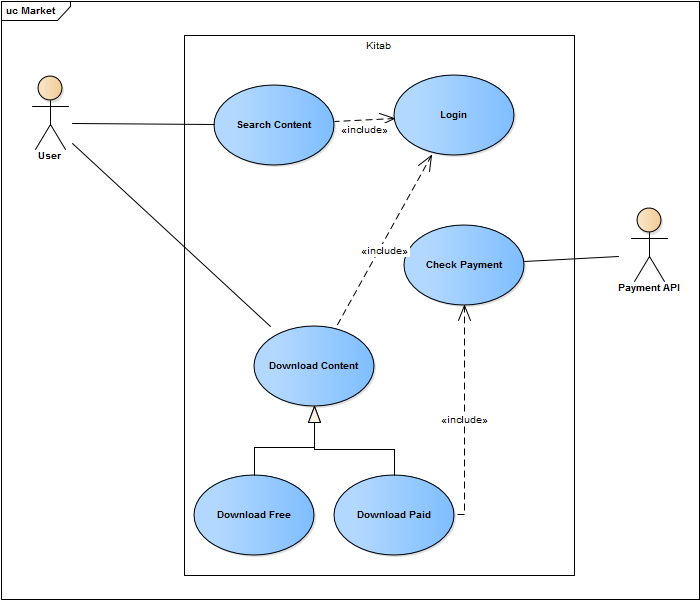
\includegraphics[width=15cm]{Diagram/Market.png}
	
	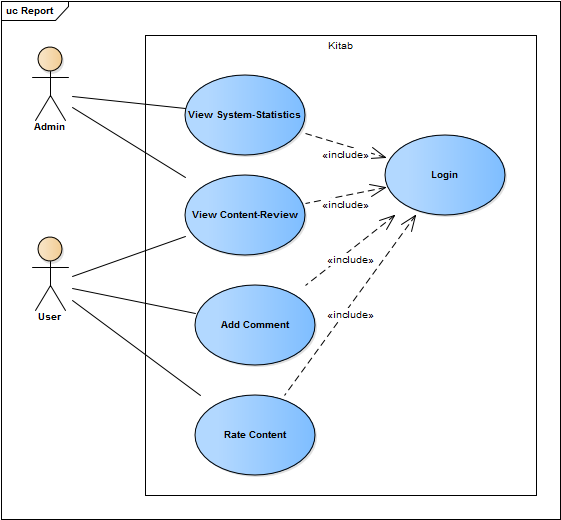
\includegraphics[width=15cm]{Diagram/Report.png}
\end{center}


	\subsection{Use-case description}



% %%%%%%%% Usecase description for Create Account
% % TODO *************************************
% \begin{table}[H]
% \begin{center}
% 	\begin{tabularx}{0.8\textwidth}{ | l | X | X | }
% 	\hline \textbf{Use-case name}
% 		& \multicolumn{2}{l |}{Create Account} \\
% 	\hline \textbf{Actor}
% 		& \multicolumn{2}{l |}{Reader, Author} \\
% 	\hline \textbf{Used Use-case}
% 		& \multicolumn{2}{l |}{Login} \\
% 	\hline \textbf{Goal of context}
% 		& \multicolumn{2}{l |}{} \\
% 	\hline \multirow{2}{*}{\textbf{Pre-condition}}
% 		& \multicolumn{2}{l |}{} \\
% 		& \multicolumn{2}{l |}{} \\
% 	\hline \textbf{Post-condition}
% 		& \multicolumn{2}{l |}{} \\
% 	\hline \textbf{Exception}
% 		& \multicolumn{2}{l |}{ } \\
% 	\hline \multirow{8}{*}{\textbf{Flow of events}}
% 		& \multicolumn{1}{c |}{\textbf{Actor}}
% 		& \multicolumn{1}{c |}{\textbf{System}} \\ \cline{2-3}
% 		& & \\
% 		& & \\
% 		& & \\
% 		& & \\
% 		& & \\
% 		& & \\
% 	\hline
% 	\end{tabularx}
% 	\caption{Use-case description template}
% \end{center}
% \end{table}



% %%%%%%%% Usecase description for Search Content

% \begin{table}[H]
% \begin{center}
% 	\begin{tabularx}{0.8\textwidth}{ | l | X | X | }
% 	\hline \textbf{Use-case name}
% 		& \multicolumn{2}{l |}{} \\
% 	\hline \textbf{Actor}
% 		& \multicolumn{2}{l |}{} \\
% 	\hline \textbf{Used Use-case}
% 		& \multicolumn{2}{l |}{} \\
% 	\hline \textbf{Goal of context}
% 		& \multicolumn{2}{l |}{} \\
% 	\hline \multirow{2}{*}{\textbf{Pre-condition}}
% 		& \multicolumn{2}{l |}{} \\
% 		& \multicolumn{2}{l |}{} \\
% 	\hline \textbf{Post-condition}
% 		& \multicolumn{2}{l |}{} \\
% 	\hline \textbf{Exception}
% 		& \multicolumn{2}{l |}{ } \\
% 	\hline \multirow{8}{*}{\textbf{Flow of events}}
% 		& \multicolumn{1}{c |}{\textbf{Actor}}
% 		& \multicolumn{1}{c |}{\textbf{System}} \\ \cline{2-3}
% 		& & \\
% 		& & \\
% 		& & \\
% 		& & \\
% 		& & \\
% 		& & \\
% 	\hline
% 	\end{tabularx}
% 	\caption{Use-case description for Search Content}
% \end{center}
% \end{table}



%%%%%%%% Usecase description for remove content

\begin{table}[H]
\begin{center}
	\begin{tabularx}{0.8\textwidth}{ | l | X | X | }
	\hline \textbf{Use-case name}
		& \multicolumn{2}{l |}{Remove content} \\
	\hline \textbf{Actor}
		& \multicolumn{2}{l |}{Admin, Author, Publisher} \\
	\hline \textbf{Used Use-case}
		& \multicolumn{2}{l |}{Login} \\
	\hline \textbf{Goal of context}
		& \multicolumn{2}{l |}{To remove unwanted content from the system} \\
	\hline \multirow{2}{*}{\textbf{Pre-condition}}
		& \multicolumn{2}{l |}{The actor must have account} \\
		& \multicolumn{2}{l |}{The actor must log into the system using his/her account} \\
	\hline \textbf{Post-condition}
		& \multicolumn{2}{l |}{The content will be removed from the system} \\
	\hline \textbf{Exception}
		& \multicolumn{2}{l |}{ } \\
	\hline \multirow{8}{*}{\textbf{Flow of events}}
		& \multicolumn{1}{c |}{\textbf{Actor}}
		& \multicolumn{1}{c |}{\textbf{System}} \\ \cline{2-3}
		& Actor will browse into the system & Login page will be displayed. \\
		& Actor will log into the system using his/her account & Homepage will be displayed. \\
		& Actor will select remove content menu. & The system will display a page containing list of books to select from. \\
		& The actor will select E-book and order remove. & The system will remove the selected E-book.  \\
		& & The system will notify the sctor sbout the status of the removal of E-book.\\
		& & The system will redirect the actor to the home page. \\
	\hline
	\end{tabularx}
	\caption{Use-case description for removing content}
\end{center}
\end{table}



%%%%%%%% Usecase description for Download content

\begin{table}[H]
\begin{center}
	\begin{tabularx}{0.8\textwidth}{ | l | X | X | }
	\hline \textbf{Use-case name}
		& \multicolumn{2}{l |}{Download content} \\
	\hline \textbf{Actor}
		& \multicolumn{2}{l |}{User} \\
	\hline \textbf{Used Use-case}
		& \multicolumn{2}{l |}{Login Check payment} \\
	\hline \textbf{Goal of context}
		& \multicolumn{2}{l |}{To download content of the book to local storage.} \\
	\hline \multirow{2}{*}{\textbf{Pre-condition}}
		& \multicolumn{2}{l |}{The user must login with his/her account.} \\
		& \multicolumn{2}{l |}{The user must pay the price if the book is commercial.} \\
	\hline \multirow{2}{*}{\textbf{Post-condition}}
		& \multicolumn{2}{l |}{The system will provide the content.} \\
		& \multicolumn{2}{l |}{The user will download the content} \\
	\hline \multirow{3}{*}{\textbf{Exception}}
		& \multicolumn{2}{l |}{\textbf{Insufficient balance}} \\ \cline{2-3}
		& \multicolumn{2}{l |}{The system will notify the user to deposit to his.her account.} \\
		& \multicolumn{2}{l |}{The system will redirect the user to the homepage.} \\
	\hline \multirow{4}{*}{\textbf{Flow of events}}
		& \multicolumn{1}{c |}{\textbf{Actor}}
		& \multicolumn{1}{c |}{\textbf{System}} \\ \cline{2-3}
		& User browses into the system. & Login page will be displayed. \\
		& User logs into his account. & Homepage containing list of books will be displayed. \\
		& User presses the download button on the book he wants to download. & \\
	\hline \multirow{4}{*}{\textbf{Scenario}}
		& \multicolumn{2}{l |}{\textbf{Download commercial E-book}} \\ \cline{2-3}
		& User will enters his payment account details. & The system will redirect him/her to payment page. \\
		& The user will enter to token. & The payment process the payment and return token indicating payment. \\
		& The user will download the content. & The system will provide the content of the book. \\
	\hline \multirow{2}{*}{\textbf{Scenario}}
		& \multicolumn{2}{l |}{\textbf{Download free E-book}} \\ \cline{2-3}
		& The user will downlosd the content. & The system will provide the content of the E-book. \\
	\hline
	\end{tabularx}
	\caption{Use-case description for downloading content}
\end{center}
\end{table}



%%%%%%%% Usecase description for Modify Content

\begin{table}[H]
\begin{center}
	\begin{tabularx}{0.8\textwidth}{ | l | X | X | }
	\hline \textbf{Use-case name}
		& \multicolumn{2}{l |}{Modify Content} \\
	\hline \textbf{Actor}
		& \multicolumn{2}{l |}{Author, Publisher} \\
	\hline \textbf{Used Use-case}
		& \multicolumn{2}{l |}{Login} \\
	\hline \textbf{Goal of context}
		& \multicolumn{2}{l |}{To modify details about the content of an E-book} \\
	\hline \multirow{3}{*}{\textbf{Pre-condition}}
		& \multicolumn{2}{l |}{The actor must have an account.} \\
		& \multicolumn{2}{l |}{The actor must log into the system uding his/her account.} \\
		& \multicolumn{2}{l |}{There must be an E-book which responds to the user.} \\
	\hline \textbf{Post-condition}
		& \multicolumn{2}{l |}{The details of the E-book will be modified.} \\
	\hline \textbf{Exception}
		& \multicolumn{2}{l |}{ } \\
	\hline \multirow{7}{*}{\textbf{Flow of events}}
		& \multicolumn{1}{c |}{\textbf{Actor}}
		& \multicolumn{1}{c |}{\textbf{System}} \\ \cline{2-3}
		& Actor browses into the system. & Login page will be displayed. \\
		& Actor will log into the system using his/her account. & The homepage will be displayed. \\
		& Actor will select modify E-book menu. & The system will display  page containing list of  E-books which corresponds to  the Actor. \\
		& The Actor will select the E-book he/she wants to modify. & The system will display editor window containing the content of the E-book to be modified. \\
		& The Actor will modify the content and press save button. & The system will update content of the E-book in the database according to the user modification. \\
		& & The system will redirect the author to the home page. \\
	\hline
	\end{tabularx}
	\caption{Use-case description for modifying content.}
\end{center}
\end{table}


%%%%%%%% Usecase description for Upload Content

\begin{table}[H]
\begin{center}
	% \begin{tabular}{ | l | p{0.3\textwidth} | p{0.3\textwidth} | }
	\begin{tabularx}{\linewidth}{ | l | X | X | }
	% \begin{tabular}{ | l | l | l | }
	\hline \textbf{Use-case name}
		& \multicolumn{2}{l |}{Upload content} \\
	\hline \textbf{Actor}
		& \multicolumn{2}{l |}{Author, Publisher} \\
	\hline \textbf{Used Use-case}
		& \multicolumn{2}{l |}{Login} \\
	\hline \textbf{Goal of context}
		& \multicolumn{2}{l |}{To upload E-book to the system} \\
	\hline \multirow{2}{*}{\textbf{Pre-condition}}
		& \multicolumn{2}{l |}{The actor must have an account.} \\
		& \multicolumn{2}{l |}{The actor must log into the system using his/her account.} \\
	\hline \textbf{Post-condition}
		& \multicolumn{2}{l |}{An E-book will be uploaded to the system.} \\
	\hline \multirow{4}{*}{\textbf{Exception}}
		& \multicolumn{2}{l |}{\textbf{Author selects file that is not valid.}} \\
		& \multicolumn{2}{l |}{The system will notify the actor about the situation.} \\
		& \multicolumn{2}{l |}{The system will offer the actor a choice whether to upload another file of go to homepage.} \\
		& \multicolumn{2}{l |}{The system will redirect the author to homepage or openfile chooser based on actor's choice.} \\
	\hline \multirow{8}{*}{\textbf{Flow of events}}
		& \multicolumn{1}{c |}{\textbf{Actor}}
		& \multicolumn{1}{c |}{\textbf{System}} \\ \cline{2-3}
		& Actor will browse into the system &  Log in page will be dis-played. \\
		& Actor will log into the system using his/her account & The homepage will be dis- played. \\
		& Actor will select upload content menu. & The system will display file chooser \\
		& The Actor will select a file and order upload of content. &  The system will convert the file to a format that is selected for the system \\
		& & The system will store the content in the database. \\
		& & The system show status of upload. \\
		& & The system will redirect the Actor to the home page. \\
	\hline
	% \end{tabular}
	\end{tabularx}
	\caption{Use-case description for uploading content}
\end{center}
\end{table}



%%%%%%%% Usecase description for Add Publisher

\begin{table}[H]
\begin{center}
	\begin{tabularx}{0.8\textwidth}{ | l | X | X | }
	\hline \textbf{Use-case name}
		& \multicolumn{2}{l |}{Add Publisher} \\
	\hline \textbf{Actor}
		& \multicolumn{2}{l |}{Admin} \\
	\hline \textbf{Used Use-case}
		& \multicolumn{2}{l |}{Login} \\
	\hline \textbf{Goal of context}
		& \multicolumn{2}{l |}{To add publisher to the system.} \\
	\hline \multirow{2}{*}{\textbf{Pre-condition}}
		& \multicolumn{2}{l |}{The admin must have his/her unique account.} \\
		& \multicolumn{2}{l |}{The admin must login using his/her unique account.} \\
	\hline \textbf{Post-condition}
		& \multicolumn{2}{l |}{A publisher will be added to the system.} \\
	\hline \multicolumn{1}{c |}{\textbf{Exception}}
		& \multicolumn{2}{l |}{\textbf{Publisher already registered to the system.}} \\
		% & \multicolumn{2}{l |}{The system will inform the admin and offer a choice to cancel registration or to enter again.} \\
		% & \multicolumn{2}{l |}{The admin will choose to enter again or to cancel registration.} \\
		% & \multicolumn{2}{l |}{The system will redirect to the add publisher form or to the homepage based on the admin choice.} \\
	\hline \multirow{7}{*}{\textbf{Flow of events}}
		& \multicolumn{1}{c |}{\textbf{Actor}}
		& \multicolumn{1}{c |}{\textbf{System}} \\ \cline{2-3}
		& Admin browses into the system. & log in page will be dis-played. \\
		& Admin logs into the system using his/her account. & The homepage will be dis- played. \\
		& Admin will select add pub- lisher menu. & The system will display form for adding publisher. \\
		& The Admin will fill in the publisher information in the form and order addition of publisher. & The system will store the publisher’s information to the database \\
		& & The system will notify the admin about the addition of publisher. \\
		& & The system will redirect the admin to the home page. \\
	\hline
	\end{tabularx}
	\caption{Use-case description for adding publisher}
\end{center}
\end{table}



% %%%%%%%% Usecase description template

% \begin{table}[H]
% \begin{center}
% 	\begin{tabularx}{0.8\textwidth}{ | l | X | X | }
% 	\hline \textbf{Use-case name}
% 		& \multicolumn{2}{l |}{} \\
% 	\hline \textbf{Actor}
% 		& \multicolumn{2}{l |}{} \\
% 	\hline \textbf{Used Use-case}
% 		& \multicolumn{2}{l |}{} \\
% 	\hline \textbf{Goal of context}
% 		& \multicolumn{2}{l |}{} \\
% 	\hline \multirow{2}{*}{\textbf{Pre-condition}}
% 		& \multicolumn{2}{l |}{} \\
% 		& \multicolumn{2}{l |}{} \\
% 	\hline \textbf{Post-condition}
% 		& \multicolumn{2}{l |}{} \\
% 	\hline \textbf{Exception}
% 		& \multicolumn{2}{l |}{ } \\
% 	\hline \multirow{8}{*}{\textbf{Flow of events}}
% 		& \multicolumn{1}{c |}{\textbf{Actor}}
% 		& \multicolumn{1}{c |}{\textbf{System}} \\ \cline{2-3}
% 		& & \\
% 		& & \\
% 		& & \\
% 		& & \\
% 		& & \\
% 		& & \\
% 	\hline
% 	\end{tabularx}
% 	\caption{Use-case description template}
% \end{center}
% \end{table}



%%%%%%%% Usecase description for Get help

\begin{table}[H]
\begin{center}
	\begin{tabularx}{0.8\textwidth}{ | l | X | X | }
	\hline \textbf{Use-case name}
		& \multicolumn{2}{l |}{Get help} \\
	\hline \textbf{Actor}
		& \multicolumn{2}{l |}{User} \\
	\hline \textbf{Used Use-case}
		& \multicolumn{2}{l |}{} \\
	\hline \textbf{Goal of context}
		& \multicolumn{2}{l |}{To get help how to use the system.} \\
	\hline \multirow{1}{*}{\textbf{Pre-condition}}
		& \multicolumn{2}{l |}{} \\
	\hline \textbf{Post-condition}
		& \multicolumn{2}{l |}{User gets some information.} \\
	\hline \textbf{Exception}
		& \multicolumn{2}{l |}{ } \\
	\hline \multirow{4}{*}{\textbf{Flow of events}}
		& \multicolumn{1}{c |}{\textbf{Actor}}
		& \multicolumn{1}{c |}{\textbf{System}} \\ \cline{2-3}
		& User browses into the system. & Login page will be displayed. \\
		& User will select get help menu. & Page containing information about how to use the system will be displayed. \\
		& User will see the information and close the window. & The system will redirect him/her to login page. \\
	\hline
	\end{tabularx}
	\caption{Use-case description for Get help}
\end{center}
\end{table}



%%%%%%%% Usecase for Update account details

\begin{table}[H]
\begin{center}
	% \begin{tabularx}{0.8\textwidth}{ | l | X | X | }
	\begin{tabularx}{\linewidth}{ | l | X | X | }

	\hline \textbf{Use-case name}
		& \multicolumn{2}{l |}{Update account details} \\
	\hline \textbf{Actor}
		& \multicolumn{2}{l |}{User} \\
	\hline \textbf{Used Use-case}
		& \multicolumn{2}{l |}{Login} \\
	\hline \textbf{Goal of context}
		& \multicolumn{2}{l |}{To update the account of user.} \\
	\hline \multirow{2}{*}{\textbf{Pre-condition}}
		& \multicolumn{2}{l |}{The user must have account.} \\
		& \multicolumn{2}{l |}{The user must log into the system.} \\
	\hline \textbf{Post-condition}
		& \multicolumn{2}{l |}{The account of the user will be updated.} \\
	\hline \multirow{6}{*}{\textbf{Exception}}
		& \multicolumn{2}{l |}{\textbf{The user enters a password that doesn't match the previous password.}} \\
		& \multicolumn{2}{l |}{ The system will notify the user to enter the password again for defined number of times.} \\
		& \multicolumn{2}{l |}{\textbf{The user enters incorrect password pattern.}} \\
		& \multicolumn{2}{l |}{The system will notify the user to enter the password again.} \\
		& \multicolumn{2}{l |}{\textbf{The user enters user name already in use.}} \\
		& \multicolumn{2}{l |}{The system will notify the user to try another user name} \\
	\hline \multirow{8}{*}{\textbf{Flow of events}}
		& \multicolumn{1}{c |}{\textbf{Actor}}
		& \multicolumn{1}{c |}{\textbf{System}} \\ \cline{2-3}
		& User browses into the system. & Login page will be displayed. \\
		&  User will log into the system using his/her account. & The homepage will be displayed. \\
		&  User will select update ac count menu. & A page asking to enter the previous password will be displayed \\
		& User will fill in his/her password and confirm modification. & Update account page containing form will be displayed. \\
		&  User will fill in the form and order updation. & The system will validate the user info. \\
		& & The system will update the corresponding account in the database. \\
		& & The system will notify the User about status of modification and redirect the user to homepage. \\
	\hline
	\end{tabularx}
	\caption{Use-case description for updating account-details }
\end{center}
\end{table}



%%%%%%%% Usecase description for Remove account

\begin{table}[H]
\begin{center}
	\begin{tabularx}{0.8\textwidth}{ | l | X | X | }
	\hline \textbf{Use-case name}
		& \multicolumn{2}{l |}{Remove account} \\
	\hline \textbf{Actor}
		& \multicolumn{2}{l |}{Reader, Author, Publisher, Admin} \\
	\hline \textbf{Used Use-case}
		& \multicolumn{2}{l |}{Login} \\
	\hline \textbf{Goal of context}
		& \multicolumn{2}{l |}{To remove user account} \\
	\hline \multirow{2}{*}{\textbf{Pre-condition}}
		& \multicolumn{2}{l |}{The actor must have his/her unique account.} \\
		& \multicolumn{2}{l |}{The actor must log into his account.} \\
	\hline \textbf{Post-condition}
		& \multicolumn{2}{l |}{User account will be removed} \\
	\hline \textbf{Exception}
		& \multicolumn{2}{l |}{ } \\
	\hline \multirow{5}{*}{\textbf{Flow of events}}
		& \multicolumn{1}{c |}{\textbf{Actor}}
		& \multicolumn{1}{c |}{\textbf{System}} \\ \cline{2-3}
		& Actor browses into the system & Login page will be displayed. \\
		& Actor will log into the system using his/her account. & The homepage will be displayed. \\
		& Actor will select remove select account. & The system will display a window asking the actor to confirm his/her password. \\
		& Actor will enter his/her password and confirm removal of his/her account. & Actor will enter his/her password and confirm removal of account. \\
	\hline \multirow{3}{*}{\textbf{Scenario}}
		& \multicolumn{2}{c |}{\textbf{'User' removes his/her account.}} \\ \cline{2-3}
		& Actor browses into the system & Login page will be displayed. \\
		& Actor will log into the system using his/her account. & The homepage will be displayed. \\
	\hline \multirow{5}{*}{\textbf{Scenario}}
		& \multicolumn{2}{c |}{\textbf{Admin removes his/her account.}} \\ \cline{2-3}
		& & The system will display a page containing a list of accounts to select from. \\
		& The Admin will select accounts to be deleted and order deletion. & The system will remove the selected accounts from the database. \\
		& & The system will notify the Admin about the deletion status. \\
		& & The system will redirect the Admin to the home page. \\
	\hline
	\end{tabularx}
	\caption{Use-case description for Remove account}
\end{center}
\end{table}



%%%%%%%% Usecase description for Login

\begin{table}[H]
\begin{center}
	\begin{tabularx}{0.8\textwidth}{ | l | X | X | }
	\hline \textbf{Use-case name}
		& \multicolumn{2}{l |}{Login} \\
	\hline \textbf{Actor}
		& \multicolumn{2}{l |}{User, Admin} \\
	\hline \textbf{Used Use-case}
		& \multicolumn{2}{l |}{Authenticate user, Recover password} \\
	\hline \textbf{Goal of context}
		& \multicolumn{2}{l |}{To log into the system.} \\
	\hline \multirow{1}{*}{\textbf{Pre-condition}}
		& \multicolumn{2}{l |}{The actor must have account.} \\
	\hline \textbf{Post-condition}
		& \multicolumn{2}{l |}{Actor logs into the system to have access.} \\
	\hline \multirow{2}{*}{\textbf{Exception}}
		& \multicolumn{2}{l |}{\textbf{Actor enters username and password that doesn't match to any account.}} \\
		& \multicolumn{2}{l |}{The system will notify the user to try again or recovery password.} \\
	\hline \multirow{3}{*}{\textbf{Flow of events}}
		& \multicolumn{1}{c |}{\textbf{Actor}}
		& \multicolumn{1}{c |}{\textbf{System}} \\ \cline{2-3}
		& Actor browses into the system. & Login page will be displayed. \\
		& Actor enters his/her user name and password and press login button & The system will redirect him/her to the homepage. \\
	\hline
	\end{tabularx}
	\caption{Use-case description for Login}
\end{center}
\end{table}



%%%%%%%% Usecase description for View system statistics

\begin{table}[H]
\begin{center}
	\begin{tabularx}{0.8\textwidth}{ | l | X | X | }
	\hline \textbf{Use-case name}
		& \multicolumn{2}{l |}{View system statistics} \\
	\hline \textbf{Actor}
		& \multicolumn{2}{l |}{Admin} \\
	\hline \textbf{Used Use-case}
		& \multicolumn{2}{l |}{Login} \\
	\hline \textbf{Goal of context}
		& \multicolumn{2}{l |}{To see the overall statistics of the system.} \\
	\hline \multirow{2}{*}{\textbf{Pre-condition}}
		& \multicolumn{2}{l |}{Admin must have account.} \\
		& \multicolumn{2}{l |}{Admin must log into the system.} \\
	\hline \textbf{Post-condition}
		& \multicolumn{2}{l |}{The statistics of the system will be reviewed.} \\
	\hline \textbf{Exception}
		& \multicolumn{2}{l |}{ } \\
	\hline \multirow{5}{*}{\textbf{Flow of events}}
		& \multicolumn{1}{c |}{\textbf{Actor}}
		& \multicolumn{1}{c |}{\textbf{System}} \\ \cline{2-3}
		& Admin will browse the system. & Login page will be displayed. \\
		& Admin will log into the system using his/her account. & The homepage will be displayed. \\
		& Admin will select an Ebook to review. & The system will show the system statistics. \\
		& Admin will review the information and close the window. & The system will redirect him/her to the homepage. \\
	\hline
	\end{tabularx}
	\caption{Use-case description for View system statistics}
\end{center}
\end{table}



%%%%%%%% Usecase description for View content review

\begin{table}[H]
\begin{center}
	\begin{tabularx}{0.8\textwidth}{ | l | X | X | }
	\hline \textbf{Use-case name}
		& \multicolumn{2}{l |}{View content review} \\
	\hline \textbf{Actor}
		& \multicolumn{2}{l |}{User} \\
	\hline \textbf{Used Use-case}
		& \multicolumn{2}{l |}{Login} \\
	\hline \textbf{Goal of context}
		& \multicolumn{2}{l |}{To review a brief information about an Ebook.} \\
	\hline \multirow{2}{*}{\textbf{Pre-condition}}
		& \multicolumn{2}{l |}{The user must have account.} \\
		& \multicolumn{2}{l |}{The user must log into the system.} \\
	\hline \textbf{Post-condition}
		& \multicolumn{2}{l |}{User will have a brief information about an Ebook.} \\
	\hline \textbf{Exception}
		& \multicolumn{2}{l |}{ } \\
	\hline \multirow{5}{*}{\textbf{Flow of events}}
		& \multicolumn{1}{c |}{\textbf{Actor}}
		& \multicolumn{1}{c |}{\textbf{System}} \\ \cline{2-3}
		& User will browse the system. & Login page will be displayed. \\
		& User will log into the system using his/her account. & The homepage will be displayed. \\
		& User will select an Ebook to review. & The system will show information about the Ebook in separate window. \\
		& User will review the information and close the window. & The system will redirect him/her to the homepage. \\
	\hline
	\end{tabularx}
	\caption{Use-case description for View content review}
\end{center}
\end{table}



%%%%%%%% Usecase description for comment and rate content

\begin{table}[H]
\begin{center}
	\begin{tabularx}{0.8\textwidth}{ | l | X | X | }
	\hline \textbf{Use-case name}
		& \multicolumn{2}{l |}{Comment and rate content} \\
	\hline \textbf{Actor}
		& \multicolumn{2}{l |}{User} \\
	\hline \textbf{Used Use-case}
		& \multicolumn{2}{l |}{Login} \\
	\hline \textbf{Goal of context}
		& \multicolumn{2}{l |}{To give feedback to authors and publishers.} \\
	\hline \multirow{2}{*}{\textbf{Pre-condition}}
		& \multicolumn{2}{l |}{The user must have account.} \\
		& \multicolumn{2}{l |}{The user must log into the system.} \\
	\hline \multirow{2}{*}{\textbf{Post-condition}}
		& \multicolumn{2}{l |}{The user will rate the content of an E-book.} \\
		& \multicolumn{2}{l |}{The user will give comment on the content of an E-book} \\
	\hline \textbf{Exception}
		& \multicolumn{2}{l |}{ } \\
	\hline \multirow{6}{*}{\textbf{Flow of events}}
		& \multicolumn{1}{c |}{\textbf{Actor}}
		& \multicolumn{1}{c |}{\textbf{System}} \\ \cline{2-3}
		& User will browse the system. & Login page will be displayed. \\
		& Use will log into the system using account. & The homepage will be displayed. \\
		& User will select comment or rate menu. & The system will display a page for giving feedback. \\
		& User will add comment or rate an Ebook. & The system will redirect the user to the hompage. \\
		& User will close windo & \\
	\hline
	\end{tabularx}
	\caption{Use-case description for Comment and rate content}
\end{center}
\end{table}


%%%%%%%% Usecase description for View account detail
 
\begin{table}[H]
\begin{center}
	\begin{tabularx}{0.8\textwidth}{ | l | X | X | }
	\hline \textbf{Use-case name}
		& \multicolumn{2}{l |}{View account detail} \\
	\hline \textbf{Actor}
		& \multicolumn{2}{l |}{User} \\
	\hline \textbf{Used Use-case}
		& \multicolumn{2}{l |}{Login} \\
	\hline \textbf{Goal of context}
		& \multicolumn{2}{l |}{To review the details of his/her account.} \\
	\hline \multirow{2}{*}{\textbf{Pre-condition}}
		& \multicolumn{2}{l |}{The user must have account} \\
		& \multicolumn{2}{l |}{The user must log into the system.} \\
	\hline \textbf{Post-condition}
		& \multicolumn{2}{l |}{User will review the details of his/her account.} \\
	\hline \textbf{Exception}
		& \multicolumn{2}{l |}{ } \\
	\hline \multirow{6}{*}{\textbf{Flow of events}}
		& \multicolumn{1}{c |}{\textbf{Actor}}
		& \multicolumn{1}{c |}{\textbf{System}} \\ \cline{2-3}
		& User will browse the system. & Log in page will be displayed. \\
		& User will log into the system using his/her account &The homepage will be displayed \\
		& User will select review account & The system will display a page containing details of user's account. \\
		& User will review details of his/her account. & The system will redirect the user to the homepage. \\
		& User will close the window. & \\
	\hline
	\end{tabularx}
	\caption{Use-case description for View account detail}
\end{center}
\end{table}

	\subsection{Activity diagram}

	
An activity diagram describes the control flow from a start point to a finish point showing the various decision paths that exist while the activity is being executed.The activity diagram for Kitab is categorized based on the Actor.


\begin{figure}[H]
\begin{center}	

	\tcbox{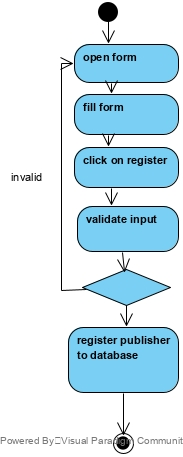
\includegraphics[width=0.4\textwidth]{Diagram/activity/Add Publisher.png}}
	\caption{Activity diagram for adding publisher.}
	\label{dia_actvt_addpblshr}

\end{center}
\end{figure}

\begin{figure}[H]
\begin{center}	

	\tcbox{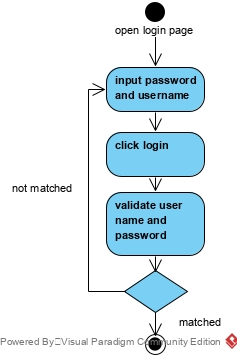
\includegraphics[width=0.6\textwidth]{Diagram/activity/Login.png}}
	\caption{Activity diagram for login.}
	\label{dia_actvt_login}

\end{center}
\end{figure}

\begin{figure}[H]
\begin{center}	

	\tcbox{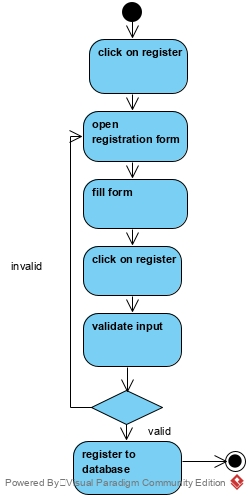
\includegraphics[width=0.6\textwidth]{Diagram/activity/Register.png}}
	\caption{Activity diagram for registering.}
	\label{dia_actvt_rgstr}

\end{center}
\end{figure}

\begin{figure}[H]
\begin{center}	

	\tcbox{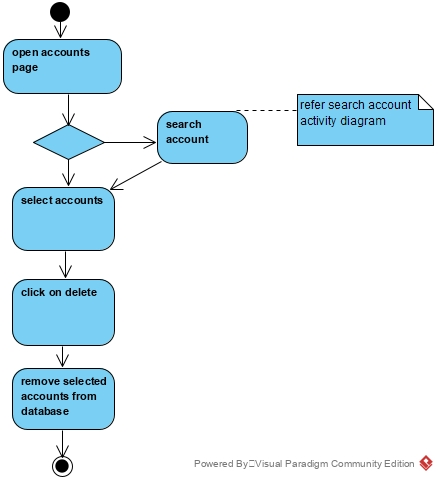
\includegraphics[width=0.6\textwidth]{Diagram/activity/Remove Account.png}}
	\caption{Activity diagram for removing account.}
	\label{dia_actvt_rmvaccnt}

\end{center}
\end{figure}

\begin{figure}[H]
\begin{center}	

	\tcbox{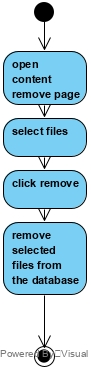
\includegraphics[width=0.2\textwidth]{Diagram/activity/Remove Content.png}}
	\caption{Activity diagram for removing content.}
	\label{dia_actvt_rmvcntnt}

\end{center}
\end{figure}

\begin{figure}[H]
\begin{center}	

	\tcbox{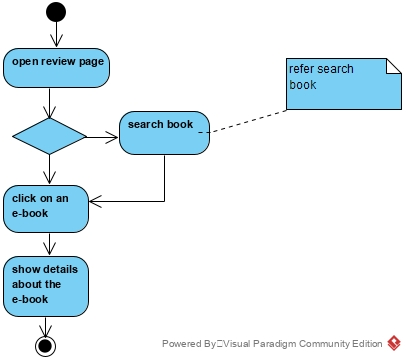
\includegraphics[width=0.6\textwidth]{Diagram/activity/Review.png}}
	\caption{Activity diagram for reviewing.}
	\label{dia_actvt_rvw}

\end{center}
\end{figure}

\begin{figure}[H]
\begin{center}	

	\tcbox{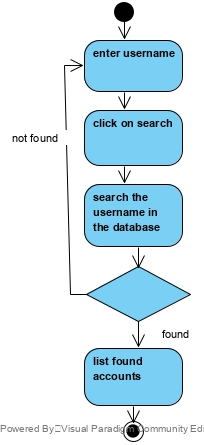
\includegraphics[width=0.4\textwidth]{Diagram/activity/Search Account.png}}
	\caption{Activity diagram for searching account.}
	\label{dia_actvt_srchaccnt}

\end{center}
\end{figure}

\begin{figure}[H]
\begin{center}	

	\tcbox{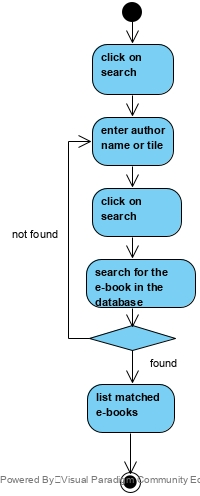
\includegraphics[width=0.4\textwidth]{Diagram/activity/Search Content.png}}
	\caption{Activity diagram for searching content.}
	\label{dia_actvt_srchcntnt}

\end{center}
\end{figure}

\begin{figure}[H]
\begin{center}	

	\tcbox{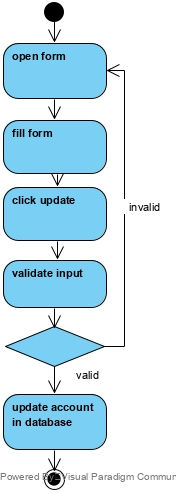
\includegraphics[width=0.4\textwidth]{Diagram/activity/Update Account.png}}
	\caption{Activity diagram for updating account.}
	\label{dia_actvt_updtaccnt}

\end{center}
\end{figure}

\begin{figure}[H]
\begin{center}	

	\tcbox{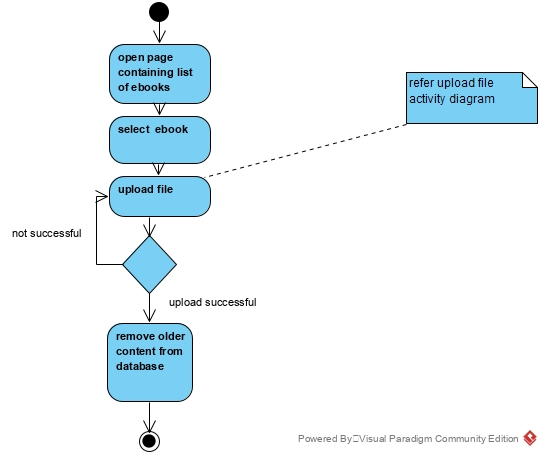
\includegraphics[width=0.6\textwidth]{Diagram/activity/Update Content.png}}
	\caption{Activity diagram for updating content.}
	\label{dia_actvt_updtcntnt}

\end{center}
\end{figure}

\begin{figure}[H]
\begin{center}	

	\tcbox{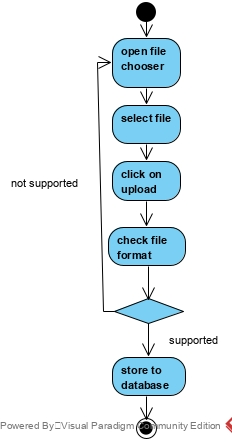
\includegraphics[width=0.6\textwidth]{Diagram/activity/Upload File.png}}
	\caption{Activity diagram for uploading file.}
	\label{dia_actvt_upldfl}

\end{center}
\end{figure}

\begin{figure}[H]
\begin{center}	

	\tcbox{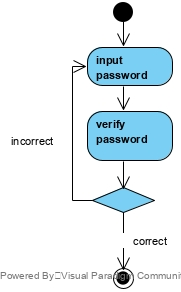
\includegraphics[width=0.6\textwidth]{Diagram/activity/Verify Password.png}}
	\caption{Activity diagram for verifying password.}
	\label{dia_actvt_vrfypsswd}

\end{center}
\end{figure}

\begin{figure}[H]
\begin{center}	

	\tcbox{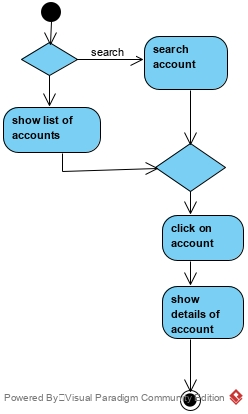
\includegraphics[width=0.6\textwidth]{Diagram/activity/View Account-details.png}}
	\caption{Activity diagram for viewing account details.}
	\label{dia_actvt_vwaccntdtls}

\end{center}
\end{figure}



































\begin{figure}[H]
\begin{center}	

	\tcbox{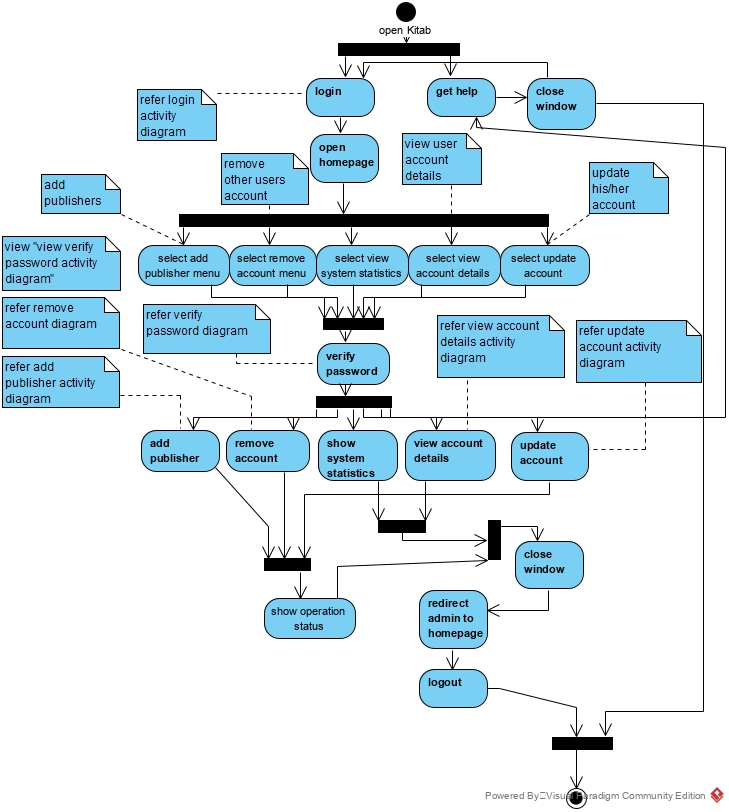
\includegraphics[width=\textwidth]{Diagram/activity/For Admin.png}}
	\caption{Activity diagram for admin.}
	\label{dia_actvt_fradmn}

\end{center}
\end{figure}

\begin{figure}[H]
\begin{center}	

	\tcbox{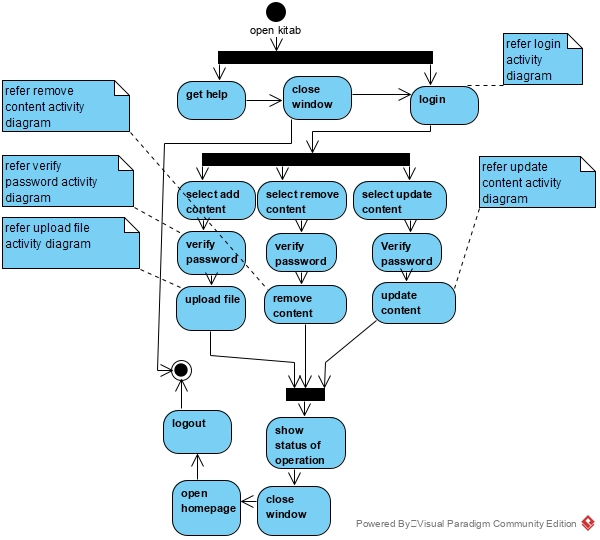
\includegraphics[width=\textwidth]{Diagram/activity/For Publisher.png}}
	\caption{Activity diagram for publisher.}
	\label{dia_actvt_frpblshr}

\end{center}
\end{figure}

\begin{figure}[H]
\begin{center}	

	\tcbox{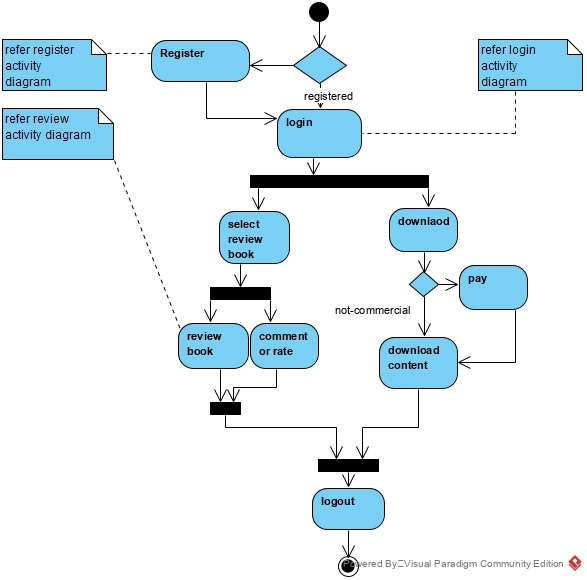
\includegraphics[width=\textwidth]{Diagram/activity/For Reader.png}}
	\caption{Activity diagram for reader.}
	\label{dia_actvt_frrdr}

\end{center}
\end{figure}



\section{Behavioural/Dynamic Modelling}

Behavioural/Dynamic modelling is a system of modeling the dynamic behavior of a system as it is executing. It shows what happens or what is supposed to happen when a system responds to a stimulus from its environment.

These stimuli may be either data or events:
	\begin{enumerate}
		\item Data becomes available that has to be processed by the system. The availability of the data triggers the processing.
		\item An event happens that triggers system processing. Events may have associated data, although this is not always the case.
	\end{enumerate}

	\subsection{Sequence diagram}

	
Sequence diagrams are Data-driven models, which are used to model interactions between system components, although external agents may also be included. A sequence diagram shows the sequence of interactions that take place during a particular use case or use case instance.

\begin{figure}[H]
\begin{center}	

	\tcbox{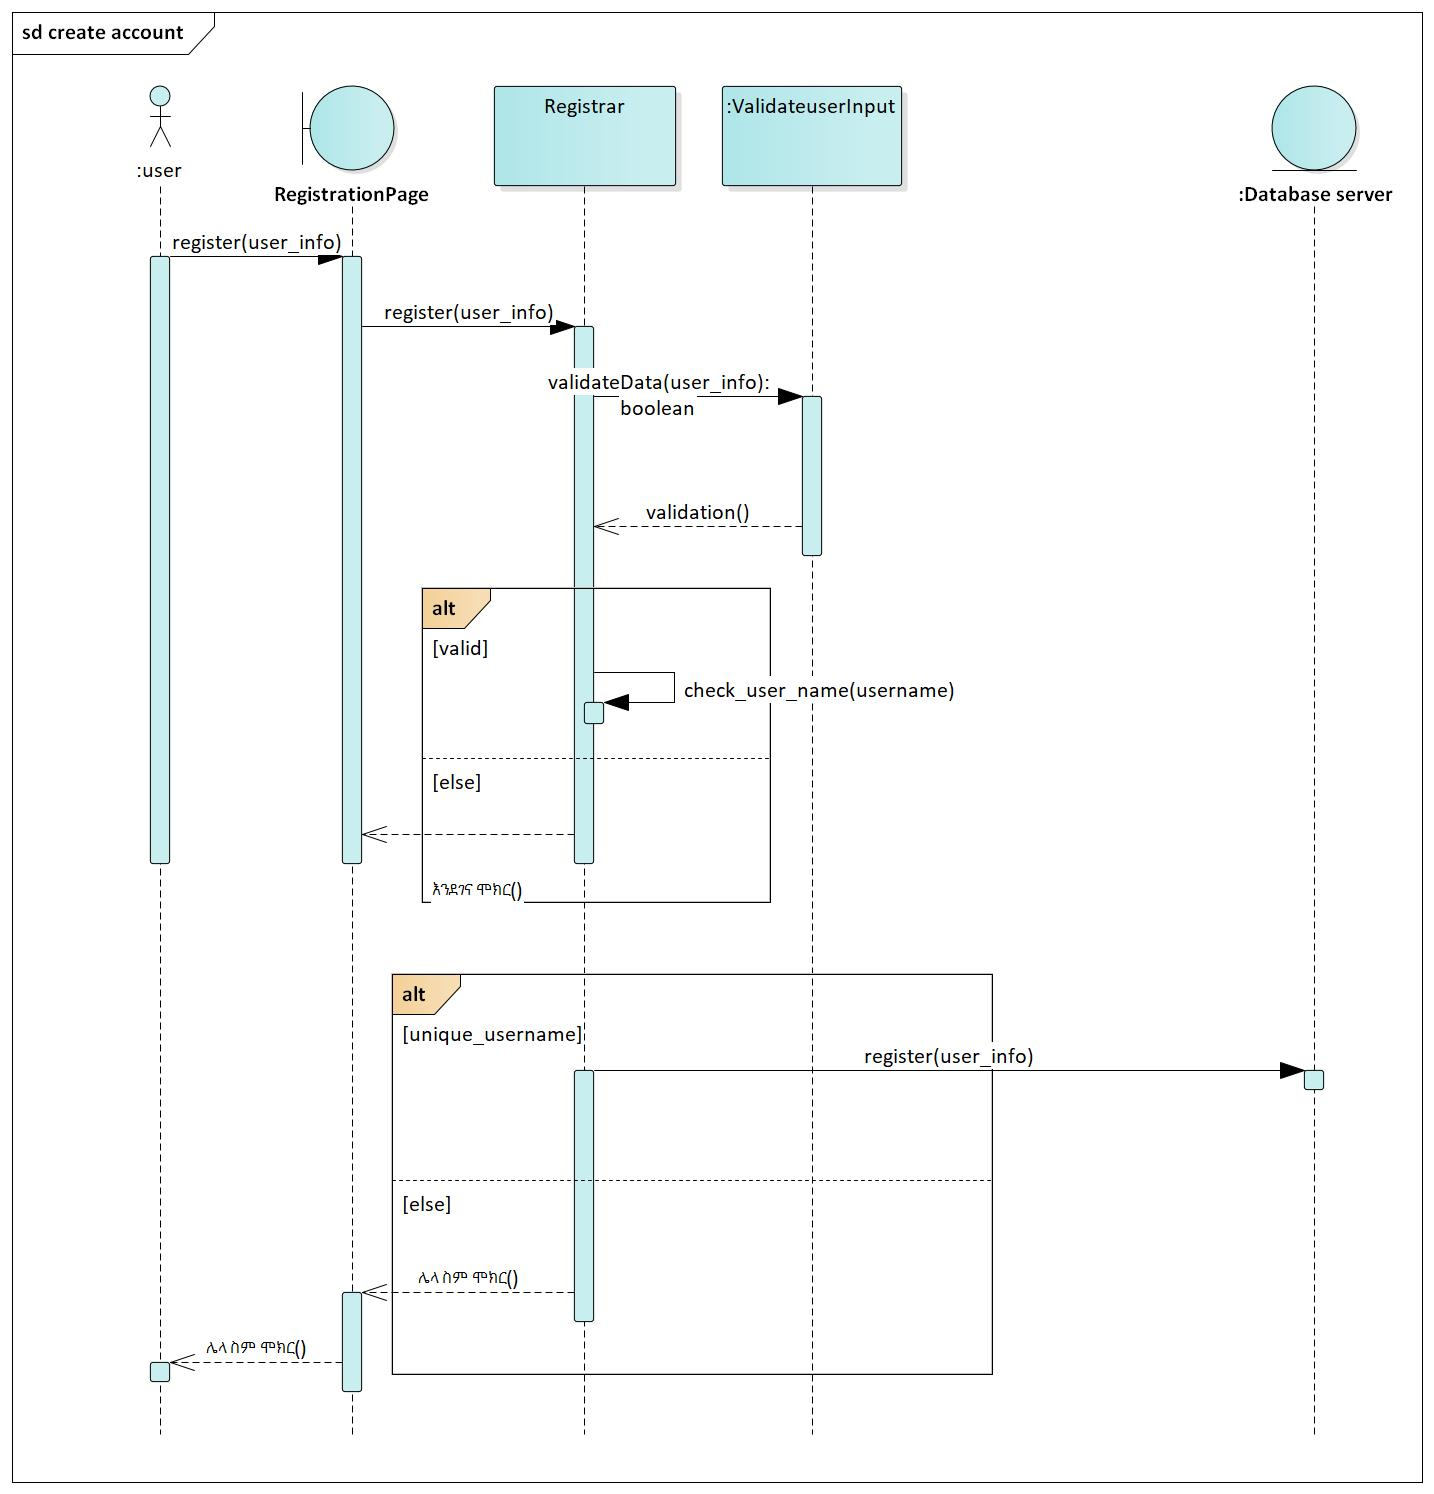
\includegraphics[width=15cm]{Diagram/sequence/Create Account.png}}
	\caption{Sequence diagram for creating account.}
	\label{dia_sqns_crtaccnt}

\end{center}
\end{figure}

\begin{figure}[H]
\begin{center}	

	\tcbox{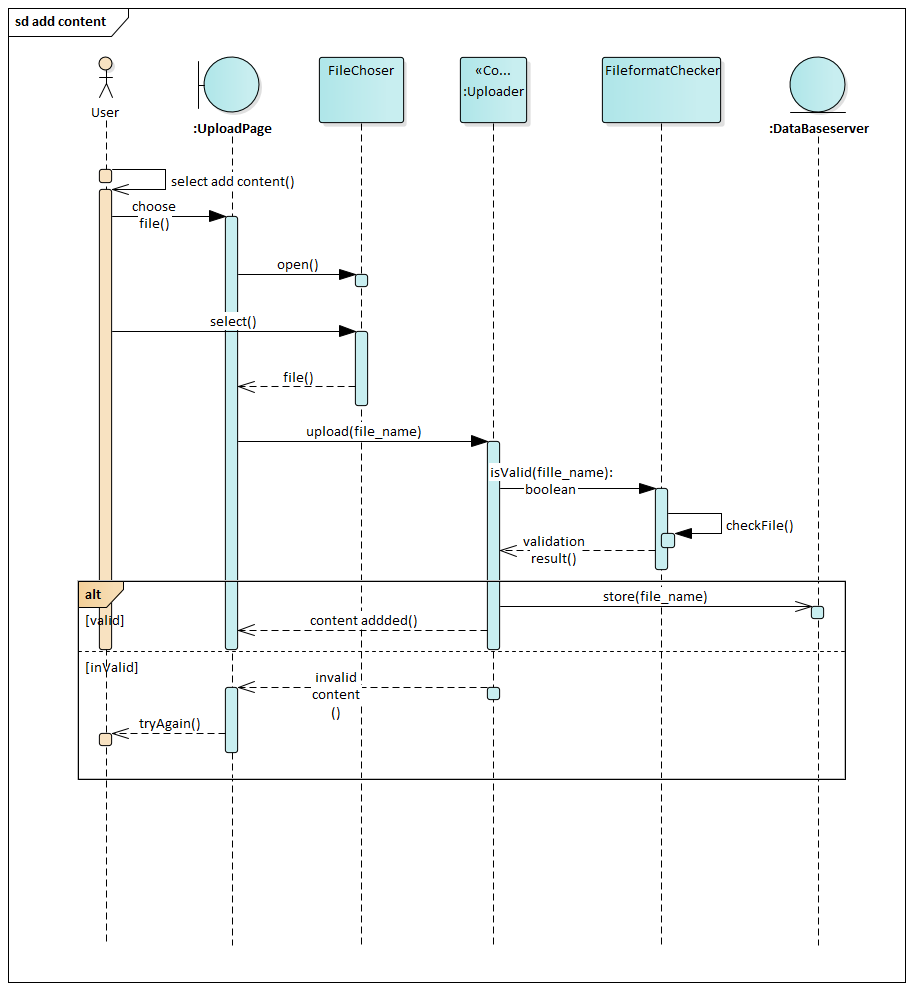
\includegraphics[width=15cm]{Diagram/sequence/Add Content.png}}
	\caption{Sequence diagram for adding content.}
	\label{dia_sqns_addcntnt}

\end{center}
\end{figure}


\begin{figure}[H]
\begin{center}	

	\tcbox{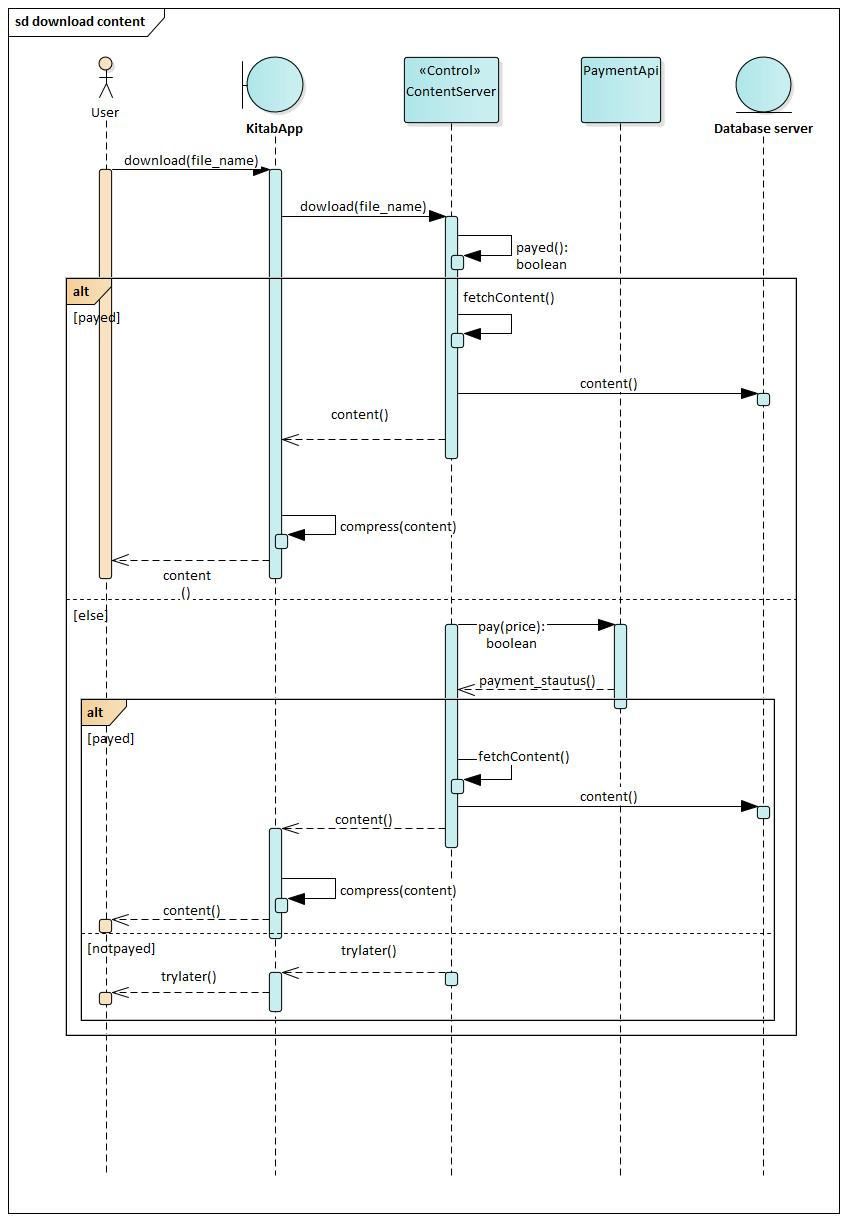
\includegraphics[width=15cm]{Diagram/sequence/Download Content.png}}
	\caption{Sequence diagram for downloading content.}
	\label{dia_sqns_dwnldcntnt}

\end{center}
\end{figure}

\begin{figure}[H]
\begin{center}	

	\tcbox{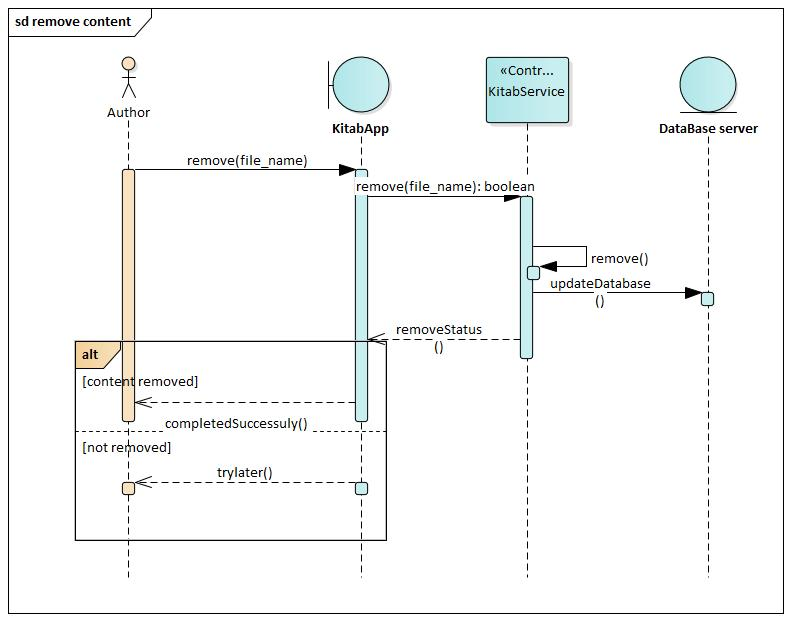
\includegraphics[width=15cm]{Diagram/sequence/Remove Content.png}}
	\caption{Sequence diagram for removing content.}
	\label{dia_sqns_rmvcntnt}

\end{center}
\end{figure}


	\subsection{State diagram}

			  
A state diagram is an event-based modeling which used to represent the condition of the system or part of the system at finite instances of time. It's a behavioral diagram and it represents the behavior using finite state transitions.


\begin{figure}[H]
\begin{center}	

	\tcbox{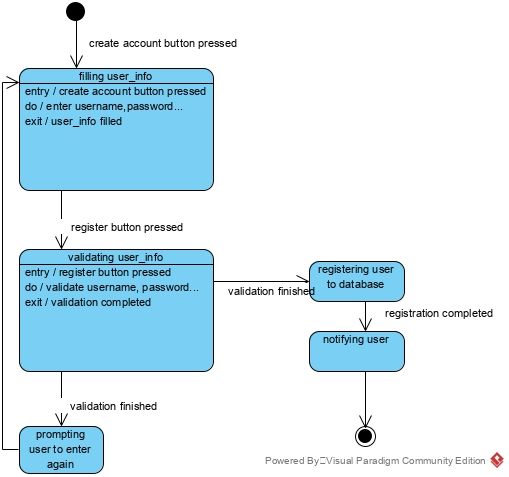
\includegraphics[width=15cm]{Diagram/state/Create Account.png}}
	\caption{State diagram for creating account.}
	\label{dia_stt_crtacnt}

\end{center}
\end{figure}

\begin{figure}[H]
\begin{center}	

	\tcbox{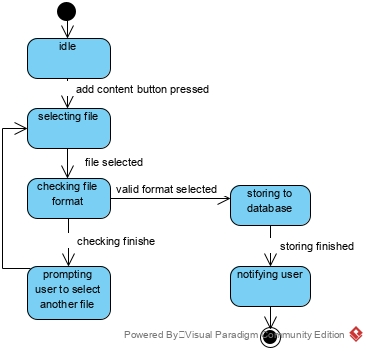
\includegraphics[width=10cm]{Diagram/state/Add Content.png}}
	\caption{State diagram for adding content.}
	\label{dia_stt_addcntnt}

\end{center}
\end{figure}

\begin{figure}[H]
\begin{center}	

	\tcbox{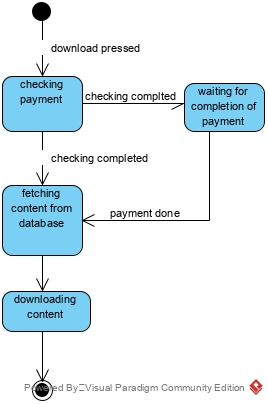
\includegraphics[width=10cm]{Diagram/state/Download Content.png}}
	\caption{State diagram for downloading content.}
	\label{dia_stt_dwnldcntnt}

\end{center}
\end{figure}

\begin{figure}[H]
\begin{center}	

	\tcbox{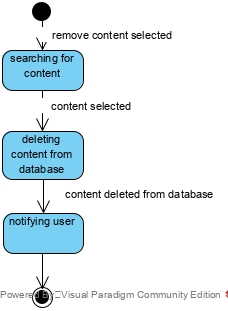
\includegraphics[width=8cm]{Diagram/state/Remove Content.png}}
	\caption{State diagram for removing content.}
	\label{dia_stt_rmvcntnt}

\end{center}
\end{figure}

   \pagebreak
   
\section{Class-Based Modeling}

Structural models of software display the organization of a system in terms of the components that make up that system and their relationships.

\textbf{Class-diagrams} for modeling the static structure of the object classes in a software system are used when developing an object-oriented system model to show the classes in a system and the associations between these classes.

	\subsection{Identifying classes}

   \begin{itemize}
   \item{User}
   \item{Content}
   \item{PaidContent}
   \item{Comment}
   \item{Address}
   \item{Admin}
   \item{Publisher}
   \item{History}
   \end{itemize}
   
   
	\subsection{Class diagram}
	
		\begin{figure}[t]
		\begin{center}
	
		\tcbox{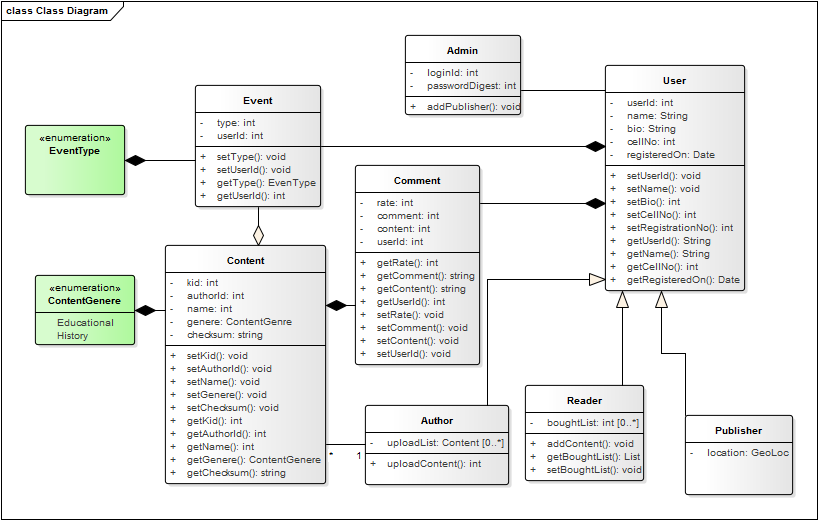
\includegraphics[angle=270, width=0.9\textwidth]{Diagram/Class Diagram.png}}
		\caption{Kitab Class diagram}
		\label{dia_class}
	
		\end{center}
		\end{figure}